\subsection{Calibration of the VMM ASIC}
\label{sec:calib_alg}

\begin{figure}[!htb]
    \begin{center}
        \includegraphics[width=0.8\textwidth]{figures/nsw/calibration/xadc_diagramPDF}
        \caption{
        }
        \label{fig:xadc_diagram}
    \end{center}
\end{figure}

As mentioned above, the VERSO software performs automated calibrations of
the frontend electronics.
The types of signals being collected on the NSW detectors are characterised by
very low signal amplitudes and are therefore typically noise dominated, with
much of the noise component derived mainly from the frontend electronics themselves.
It is therefore necessary to optimise the readout functionality of the
the VMM ASIC by calibrating it and ensuring that its signal-to-noise
ratio, $S/N$, is maximised during datataking.
Additionally, to achieve the best performance in the reconstruction of particle
tracks in the NSW detectors, several key aspects such as the charge amplitude
and timing measurement of the VMM need to be understood and well calibrated.
In this section a few of the calibration routines supported by VERSO will be discussed.

Many of the VMM calibrations rely on an external measurement of certain VMM characteristics
to be made.
These measurements are made using absolute measurements independent of any of the
internal VMM measurement mechanisms.
The VMM has built-in multiplexing capabilities that allow for it to route analog signals
to the MO output described in previous sections.
Specific for calibration, the VMM can route to MO any of the following:
\begin{description}
    \item[] \textbf{Channel Analog Output}: Analog levels of each channel's analog level prior to digitisation via the internal ADCs
    \item[] \textbf{Threshold DAC}: Analog output of the DAC controlling the global VMM threshold
    \item[] \textbf{Test Pulse DAC}: Analog output of the DAC controlling the test pulse amplitude
    \item[] \textbf{Channel Threshold Trimmers}: Analog measurement of each channel's discriminator's threshold voltage
\end{description}
On the frontend boards housing an FPGA, as in Figure~\ref{fig:frontend_boards}, the external measurement
is made by routing the MO output of a VMM to the built-in 12-bit ADC of the \textsc{Xilinx} FPGA, referred to as
the xADC.
The xADC has a full scale range of 1\,V, providing a digital measurement resolution of roughly 0.24\,mV.
The digitised samples produced by the analog measurements of the xADC are forwarded to the VERSO
DAQ software so that they can be stored and subsequently processed by the calibration algorithms.
As the xADC is housed in the on-board FPGA, the VERSO software can control its operation and access its measurements
using similar configuration and DAQ functionalities as described in the previous section.
Alternatively, the external measurement of the MO can be made via an oscilloscope probe.
The use of the oscilloscope probe does not lend itself to automated calibration but provides for
direct inspection of the analog levels as well as a reference on the measurements of the xADC.
An illustration of these external measurement mechanisms is provided in Figure~\ref{fig:xadc_diagram}.

\subsubsection{DAC Calibration}
\label{sec:calib_dac}

Each VMM has two important DACs: one for setting the global VMM threshold and one for
setting the amplitude of the injected test-pulse charge via the test-pulse capacitor on each
channel.
Each is 10-bit, meaning that it can be set to a value of 0-1023 (inclusive).
In order for the user to know in absolute terms what the VMM threshold or test-pulse amplitude
is set to, i.e. in terms of analog voltage values and not digital counts, the analog level of each
DAC is measured using the xADC.
At each configured DAC value, between 0 and 1023, analog measurements are made of the DAC output and
the relationship between the output analog value and configured digital value can be obtained.
This is illustrated in Figure~\ref{fig:threshold_dac_calib} for a single VMM's threshold DAC.
A linear relationship is assumed and from a linear fit the \textit{DAC-mV} relation, giving
the mapping from the configured digital DAC value to its analog value observed by the VMM channels, is obtained
from the slope of the line.
The DAC-mV relation between VMMs is not necessarily the same, and therefore must be measured
for every single VMM in the system in order to be able to configure them all with the
same \textit{absolute} threshold or to inject test pulses with common amplitudes across VMMs.
Given the known capacitance of the test-pulse injection capacitor of the VMM channels,
the value of the injected charge for a configured test-pulse amplitude can be obtained via the $Q = C \cdot V$
relation, where $C$ is the injection capacitor's capacitance and $V$ is the test-pulse DAC output amplitude.%\footnote{
%The quoted capacitance value of the VMM channel's test-pulse injection capacitor, 3\,pF, is that of the
%VMM3 series of VMM. Earlier versions had lower capacitances.
%}

\begin{figure}[!htb]
    \begin{center}
        \includegraphics[width=0.6\textwidth]{figures/nsw/calibration/threshold_dac_calib}
        \caption{
            VMM global threshold measurement, using measurements made by the xADC, as a function
            of the set digital DAC value.
            The slope and y-intercept (`Constant') of the linear fit are provided.
            The slope gives the DAC-mV relation that allows for converting the digtal DAC
            configured value to an analog level at the VMM inputs.
        }
        \label{fig:threshold_dac_calib}
    \end{center}
\end{figure}

\subsubsection{Measurement of Channel Baselines and Noise}
\label{sec:calib_baselines}

External measurements via the xADC can be made of each channel's analog output (i.e. prior
to digitisation) when no signals are present at the channel input.
Doing so allows one to obtain a measurement of the channel \textit{baseline}, i.e. the
ambient level when no signal is present.
Fluctuations about the baseline, then, give a measurement of the inherent channel \textit{noise}.
Measurements of both of these quantities are important, both when the frontend electronics
are and are not interfaced to a detector.
Measurements of the noise when the frontend electronics are not interfaced to a detector give
a measurement of the inherent electronics noise characteristic of the frontend board.
Interfacing the frontend electronics to a detector introduces additional capacitive effects
that can introduce new sources of noise that must also be studied and reduced.
Knowledge of both the absolute baseline and noise levels of each VMM allows for the optimal threshold
to be set for each.
In order to be sensitive to small-amplitude signals, one would set the threshold just above the baseline
which sets the zero-level of an observable signal.
In practice, one sets the VMM threshold a few times the magnitude of the measured noise above the baseline: typically
2 to 3 times the level of the measured noise above the baseline.
Figure~\ref{fig:baselines_calib} shows an example of the measurements of a VMM channel's baseline and noise, taken by the xADC.
The xADC samples each channel's baseline and from the width of the distribution of these measurements the noise
level can be obtained.

\begin{figure}[!htb]
    \begin{center}
        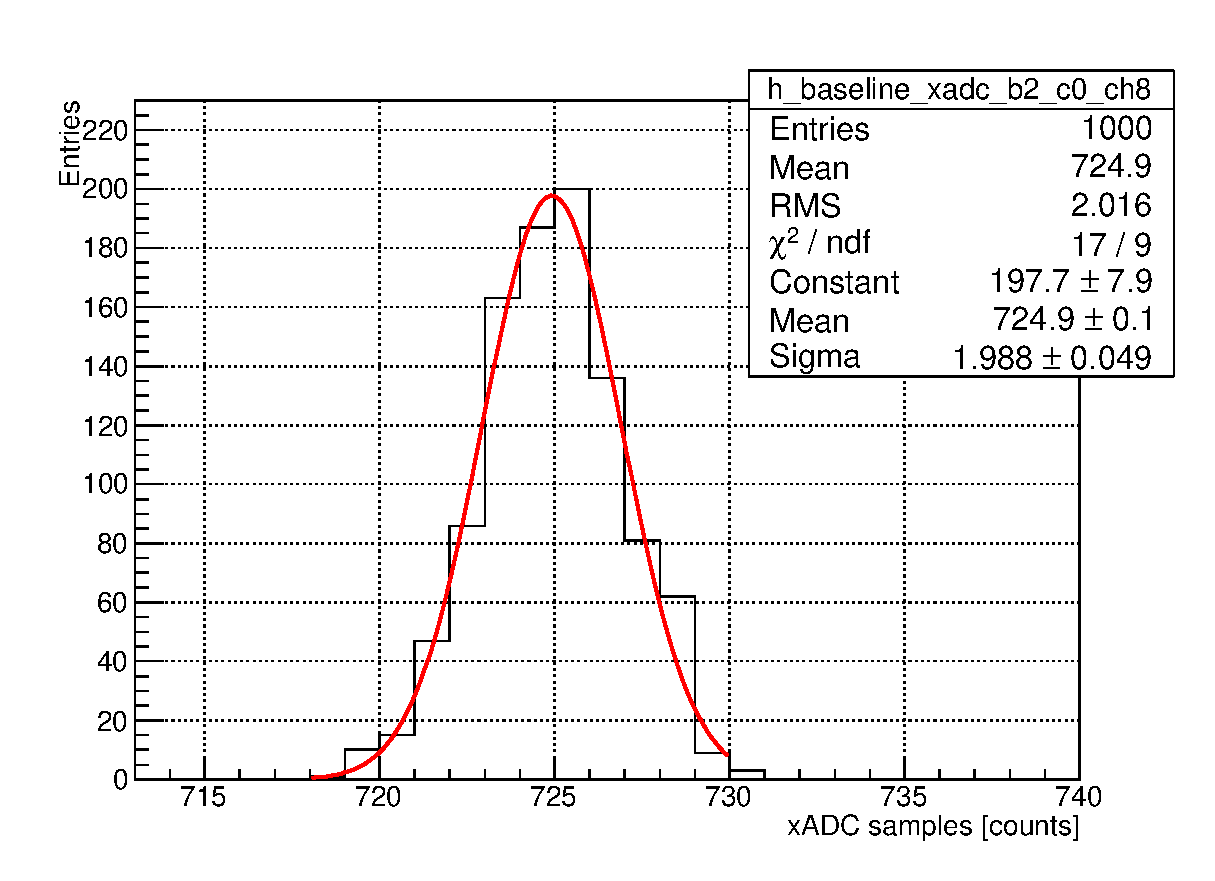
\includegraphics[width=0.46\textwidth]{figures/nsw/calibration/xadc_calib_channel_baseline_samples}
        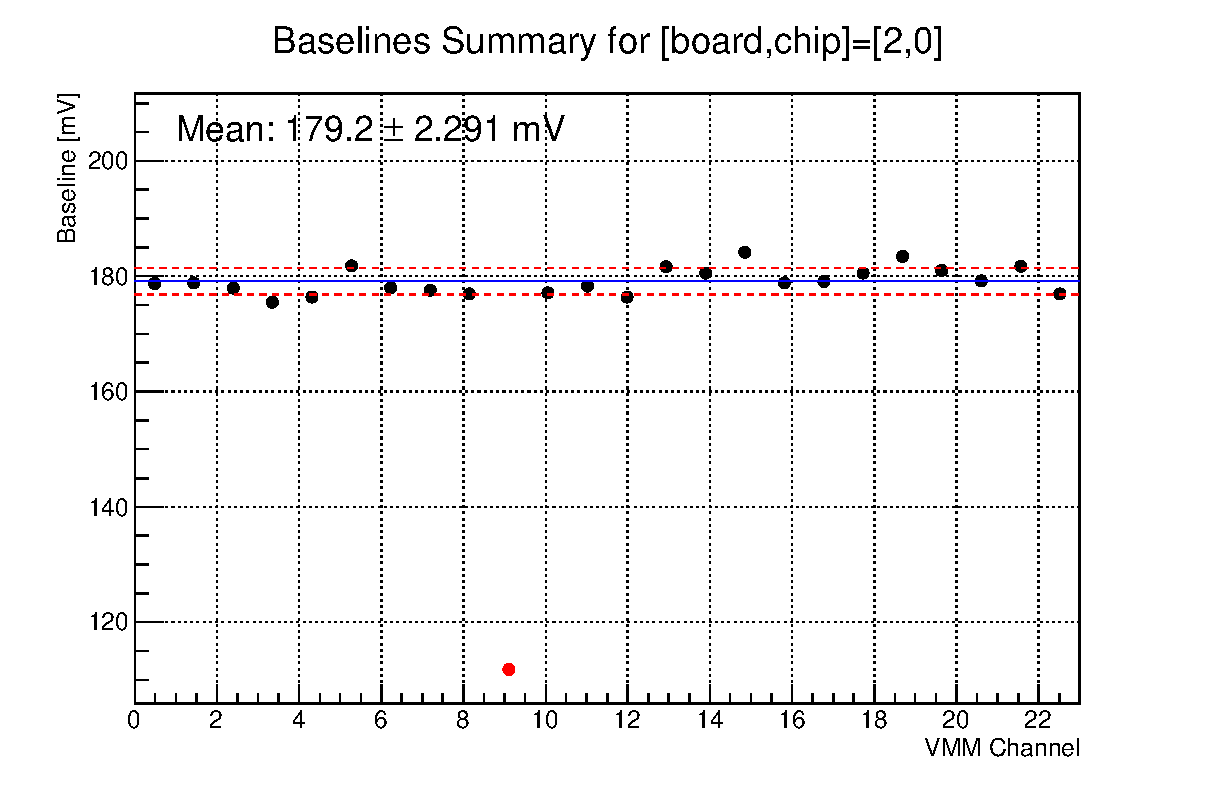
\includegraphics[width=0.53\textwidth]{figures/nsw/calibration/calib_baselines_vmm_summary}
        \caption{
            \textbf{\textit{Left}}: 1000 xADC measurements of a single VMM channel's input baseline.
                The width of the gaussian fit (red) gives the channel's noise level.
            \textbf{\textit{Right}}: Summary of the baseline measurements for 24 channels of a VMM.
                The error on the reported mean baseline, which is indicated by the blue line, is given by the RMS spread of the baseline measurements
                across all channels and is indicated by the red dashed lines.
                The channel with the red point (channel 9) is a faulty (dead) channel.
        }
        \label{fig:baselines_calib}
    \end{center}
\end{figure}

\subsubsection{Channel Threshold Trimming}
\label{sec:calib_trimming}

The global VMM threshold inherently has channel-to-channel variation.
In order to ensure that the VMM discriminators of all channels in the system
fire at the same value, the VMM has a per-channel threshold trimming functionality included.
This functionality allows for each channel's threshold to be adjusted (`trimmed') in 32 steps that cover a range
of approximately 32\,mV.
To equalize the channel discriminators, external measurements made via the xADC are performed.
For each channel, measurements of the channel discriminator's threshold are taken at each of the 32
steps in the allowed range of trimming.
Once done for every VMM channel in the system, a metric for equalizing their thresholds is needed.
In the example of Figure~\ref{fig:calib_channel_trim}, the metric is to bring all channels
as close as possible to the globally set VMM threshold.
Once this is done, all VMM channels in the system ideally have equal thresholds and will
have equivalent responses to input signals.
As seen in Figure~\ref{fig:calib_channel_trim}, prior to this calibration there is quite
some variation, which shows the importance of this fine-grained calibration procedure.
The amount of threshold trimming necessary to bring a channel to its equalized state
is independent of the globally set VMM threshold; therefore, once the calibration procedure
is performed and the subsequent channel threshold trimming is applied, the global
threshold can be adjusted with confidence that all channels in the system are likewise adjusted coherently.

\begin{figure}[!htb]
    \begin{center}
        \includegraphics[width=0.85\textwidth]{figures/nsw/calibration/channel_threshold_calibPDF}
        \caption{
            Summary plot of a VMM channel threshold trimming calibration.
            For this set up, a single VMM is calibrated and has a global threshold
            set to 235\,mV.
            The channel-by-channel variation of the threshold is seen by the yellow dots,
            which indicate the per-channel threshold measurement made by the xADC prior to any
            threshold trimming.
            The blue columns indicate the entire threshold range accessible by each channel
            by scanning the full range of channel trimmers and taking xADC measurements at each.
            It can be seen that most channels have a full range of approximately 32\,mV.
            The calibration algorithm shown here picks for all VMM channels the amount of trimming
            that allows for them to have thresholds as near as possible to the globally set threshold.
            In this case, the post-calibration threshold of all channels, indicated by the red dots,
            is very nearly 235\,mV, and is $234.8\pm 0.27$\,mV on average.
        }
        \label{fig:calib_channel_trim}
    \end{center}
\end{figure}

\subsubsection{Signal Amplitude Gain and Pedestal}
\label{sec:calib_pdo}

\subsubsection{Timing Measurement Calibration}
\label{sec:calib_tod}

